\subsection{The $p^*$ approximation in exponential families} \label{sec-pstar}

Next, we apply the Saddlepoint approximation to an exponential family $\mathcal{P} = \left\{P_\theta\right\}_{\theta}$ with natural parameter $\theta \in \Rp$. We write $f(\cdot; \theta)$ for the density of $P_\theta \in \mathcal{P}$. Then, $f(\cdot; \theta)$ is given by
\begin{equation*}
    f(x; \theta) = \expf{\theta^\top T(x) - \mathcal{H}(\theta) - \mathcal{G}(x)}.
\end{equation*}
Given a random sample $x = (x_1, \ldots, x_n)$ of $P_\theta$, the \textit{log-likelihood function} denoted $\ell(\cdot; x)$ is given by
\begin{equation*}
    \ell(\theta; x) = \theta^\top \sum_{i=1}^n T(x_i) - n \mathcal{H}(\theta) = n\left[\bar t - \mathcal{H}(\theta)\right],
\end{equation*}
where $\bar t = n^{-1}\sum_{i=1}^n T(x_i)$ is the sample average of the sufficient statistic. Hence, the maximum likelihood estimator of $\theta$ is the value $\hat\theta_{\bar t} \in \Rp$ satisfying the score equation
\begin{equation} \label{eq-score-expfam}
    \mathcal{H}'(\hat\theta_{\bar t}) = \bar t.
\end{equation}
For simplicity, we will assume that $\mathcal{H}'$ is one-to-one to ensure that (\ref{eq-score-expfam}) has a unique solution $\hat\theta_{\bar t}$. In the exponential family $\mathcal{P}$, it can be shown that the cumulant generating function of any member $P_\theta \in \mathcal{P}$ is given by $K_\theta(t) = \mathcal{H}(\theta + t) - \mathcal{H}(\theta)$. Thus $K'_\theta(t) = \mathcal{H}'(\theta + t)$. Using the cumulant generating function in the score equation (\ref{eq-score-expfam}) gives
\begin{equation*}
    K'_\theta(\hat\theta_{\bar t} - \theta) = \bar t.
\end{equation*}
Consider the Saddlepoint equation given in (\ref{eq-saddlepoint}), and notice that the parameter $\hat\gamma_{\bar t}$ of the tilted family nearly corresponds to the maximum likelihood estimator $\hat\theta$ with
\begin{equation*}
    \hat\gamma_{\bar t}/n = \hat\theta_{\bar t} - \theta.
\end{equation*}
Using this in the first order Saddlepoint approximation (\ref{eq-saddle-3}), we obtain that the Saddlepoint approximation for the average $\bar T = n^{-1}\sum_{i=1}^n T(X_i)$, where $X_1, \ldots, X_n \simiid P_\theta$, is
\begin{align*}
    g(\bar t; K_\theta) 
    &= \left(\frac{n}{2\pi}\right)^{p/2}|K_\theta''(\hat\theta_{\bar t} - \theta)|^{-1/2} \expf{nK_\theta(\hat\theta_{\bar t} - \theta) - (\hat\theta_{\bar t} - \theta)^\top \bar t}\\
    &= \left(\frac{n}{2\pi}\right)^{p/2}|\mathcal{H}''(\hat\theta_{\bar t})|^{-1/2} \expf{n(\mathcal{H}(\hat\theta_{\bar t}) - \mathcal{H}(\theta)) - (\hat\theta_{\bar t} - \theta)^\top \bar t}\\
    &= \left(\frac{n}{2\pi}\right)^{p/2}|j(\hat\theta_{\bar t})|^{-1/2} \expf{\ell(\theta; \bar t) - \ell(\hat\theta_{\bar t}; \bar t)},
\end{align*}
where the last equality follows from the fact that $\mathcal{H}''(\hat\theta)$ is equal to the observed Fisher information $j(\hat\theta)$. Daniels \cite{daniels1958} notes that this approximation can further be used to approximate the distribution of the maximum likelihood estimator. Let $\hat\Theta$ be the random variable solving the score equation $\mathcal{H}'(\hat\Theta) = \bar T$. By change of variable, we can use the approximation above to construct an approximation $p^*$ to the distribution of $\hat\Theta$ and obtain that 
\begin{equation*}
    p^*(\hat\theta; \theta, \bar t) = \left(\frac{n}{2\pi}\right)^{p/2}|j(\hat\theta)|^{-1/2} \expf{\ell(\theta; \bar t) - \ell(\hat\theta; \bar t)} \abs{\frac{\d \hat\theta}{\d \bar t}}^{-1}.
\end{equation*}
To compute the determinant of the Jacobian of the transformation $\hat\theta(\bar t)$, we  differentiate the score equation with respect to $\hat\theta$ to find $\mathcal{H}''(\hat\theta) = (\d \bar t / \d \hat\theta)$ and hence $(\d \hat\theta / \d \bar t) = \mathcal{H}''(\hat\theta)^{-1} = j(\hat\theta)^{-1}$. Therefore,
\begin{equation} \label{eq-pstar}
    p^*(\hat\theta; \theta, \bar t) = \left(\frac{n}{2\pi}\right)^{p/2}|j(\hat\theta)|^{1/2} \expf{\ell(\theta; \bar t) - \ell(\hat\theta; \bar t)}.
\end{equation}
While the dependence on $\bar t$ naturally comes from the proposed derivation of the $p^*$ approximation, it is often more convenient to parametrize the loglikelihood $\ell(\cdot; x)$ and $p^*$ approximations in terms of the maximum likelihood estimator $\hat\theta(\bar t)$. We then write
\begin{equation*}
    p^*(\hat\theta; \theta, \hat\theta) = \left(\frac{n}{2\pi}\right)^{p/2}|j(\hat\theta)|^{1/2} \expf{\ell(\theta; \hat\theta) - \ell(\hat\theta; \hat\theta)}.
\end{equation*}
This highlights the fact that the $p^*$ approximation inherited its locality from the Saddlepoint approximation, since the density $p^*(\hat\theta; \theta, \hat\theta)$ is different at each point $\hat\theta$ at which it is evaluated. The $p^*$ approximation can also be used in many different situations where the distribution of refence is not necessarily an exponential family. Several articles and books by Barndorff-Nielsen\cite{BarndorffNielsen1980,BarndorffNielsen1983} and other authors study and derive the $p^*$ approximation in broader generality.

Suppose now that the exponential family $\mathcal{P}$ has an alternative parametrization $\{ P_\phi \}$ such that there exists a diffeomorphism $\phi = \phi(\theta)$ satisfying $\hat\phi = \phi(\hat\theta)$, where $\hat\phi$ and $\hat\theta$ are the maximum likelihood estimators in their respective parametrizations. Then, 
\begin{align*}
    p^*(\hat\phi; \phi, \hat \phi) 
&= \left(\frac{n}{2\pi}\right)^{-p/2}|j_\phi(\hat\phi)|^{1/2} \expf{\ell(\phi; \hat \phi) - \ell(\hat\phi; \hat \phi)}\\
&= \left(\frac{n}{2\pi}\right)^{-p/2}\left(|j_\theta(\theta(\hat\phi))|\abs{\frac{\d \hat\theta}{\d \hat\phi}}^{-2}\right)^{1/2} \expf{\ell(\theta(\phi); \theta(\hat \phi)) - \ell(\theta(\hat\phi); \theta(\hat \phi))}\\
&= p^*(\theta(\hat\phi); \theta(\phi), \theta(\hat \phi))\abs{\frac{\d \hat\theta}{\d \hat\phi}}^{-1}.
\end{align*}
Hence, the $p^*$ approximation is invariant under reparametrization. 

\begin{example}

    \begin{figure}[!htbp]
        \textbf{Error of $p^*$ approximation of MLE in $\t{Exp}(\lambda)$ model with $n=10$}
        \centering
        \subfloat{
            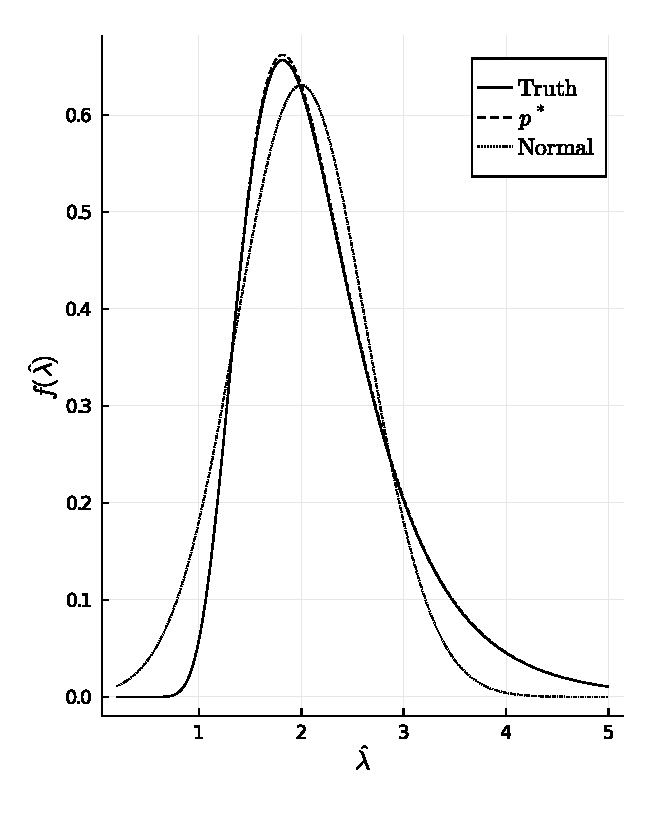
\includegraphics[width=8cm]{pstar_exp_dens.eps} 
        }
        \subfloat{
            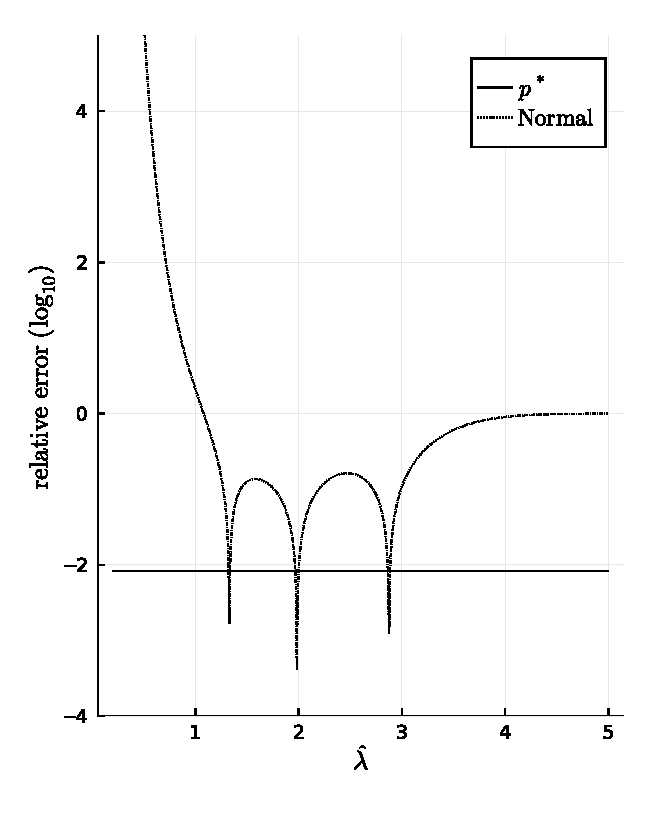
\includegraphics[width=8cm]{pstar_exp_err.eps} 
        }
        \caption{Study of the approximation error of the Saddlepoint approximation on a standardized sum of $n=10$ of $\Gamma(2, 1)$ random variables. Both panel exposes properties studied of the Saddlepoint approximation: the accurate rellative error, the gain in order of approximation and the uniform relative error of the approximation for sums of Gamma random variables.}
        \label{fig-pstar-approx}
    \end{figure}    

    We estimate the density of the maximum likelihood estimator of the parameter $\lambda \in \R_+$ of an exponential distribution $\t{Exp}(\lambda)$. The density of the distribution $\t{Exp}(\lambda)$ is
    \begin{equation*}
        f_\lambda(x) = \lambda \expf{-\lambda x}.
    \end{equation*}
    To make direct use of the $p^*$ approximation in (\ref{eq-pstar}), we must work in the natural parametrization of the exponential distribution. For $\lambda \in R_+$, the corresponding natural parameter is $\theta = -\lambda \in \R_-$ and the density of $\t{Exp}(\theta)$ is then $f_\theta(x) = \expf{ \theta x + \logf{-\theta}}$. Given an i.i.d.\,sample $x_1, \ldots, x_n$ of $\t{Exp}(\theta)$, we the log-likelihood function is given by 
    \begin{equation*}
        \ell(\theta; \bar x) = n\left[\theta \bar x + \logf{-\theta}\right],
    \end{equation*}
    where we used that the sufficient statistic is $T(x) = x$ and hence $\bar t = \bar x$ is the sample mean. The maximum likelihood estimator of $\theta$ is then $\hat\theta = -1/\bar x$ and the observed information is equal to $j(\theta) = 1/\theta^2$. Since $\t{Exp}(\lambda) = \Gamma(1, \lambda)$, the distribution of $\bar X$ is $\Gamma(n, n\lambda)$ and hence $\hat\lambda = \bar x$ is $\t{Inv-}\Gamma(n, n\lambda)$. 
    \\
    It follows that the $p^*$ approximation to the density of $\hat\theta$ is
    \begin{align*}
        p^*(\hat\theta; \theta, \hat\theta) 
        &= \sqrt{n} \frac{|\theta|^n}{|\hat\theta|^{n-1}}\expf{-n(\theta - \hat\theta)/\hat\theta} / \sqrt{2\pi}\\
        &= \sqrt{n} \frac{|\theta|^n}{|\hat\theta|^{n-1}}\expf{n\left[1 - \frac{\theta}{\hat\theta}\right]} / \sqrt{2\pi}.
    \end{align*}
    Using the invariance of the $p^*$ approximation, we obtain a $p^*$ approximation of the density of the maximum likelihood parameter $\hat\lambda$ in the original parametrization,
    \begin{align}
        p^*(\hat\lambda; \lambda, \hat\lambda) 
        &= p^*(\theta(\hat\lambda); \theta(\lambda), \theta(\hat\lambda)) \abs{\d \hat\theta / \d \hat\lambda}^{-1} \nonumber\\
        &= \sqrt{n} \frac{|\lambda|^n}{|\hat\lambda|^{n-1}}\expf{n\left[\frac{\lambda}{\hat\lambda} - 1\right]} / \sqrt{2\pi}. \label{eq-pstar-lambda}
    \end{align}
    
    The Normal approximation is a commonly used approximation to the distribution of the maximum likelihood estimator. In the exponential model, the Fisher information is $I(\lambda) = \lambda^{-2}$ and the following central limit theorem holds for the maximum likelihood estimator \cite[Example 3.12]{lehmann2006theory}
    \begin{equation} \label{eq-normal-lambda}
        \sqrt{n}(\hat\lambda - \lambda) \xrightarrow[]{\d} N(0, I(\lambda)^{-1})\ \ \ \  \t{as } n \rightarrow \infty.
    \end{equation}
    Hence, $\hat\lambda$ is approximately $N(\lambda, \lambda^2/n)$ with an approximation error of the density of $O(n^{-1/2})$. 
    
    In Figure \ref{fig-pstar-approx}, we display how (\ref{eq-pstar-lambda}) and (\ref{eq-normal-lambda}) approximate the density of $\hat\lambda$ under the true model $\t{Exp}(2)$. As we can see in the left panel, the $p^*$ approximation properly fits the true density of $\hat\lambda$ and captures the bias of the $\hat\lambda$ estimator as opposed to the Normal approximation which is centered around the true value of $\lambda$. Furthermore, we observe in the right panel how the relative error of the $p^*$ approximation is identical to the approximation error of the Saddlepoint approximation to the mean of $\Gamma(2, 1)$ seen in Example \ref{ex-gamma-saddle}. This is also a direct consequence of the invariance of the $p^*$ approximation since $\hat\Lambda$, the random variable associated to the MLE, is the inverse of the sample mean $\bar X$, which is a diffeomorphic transformation for positive reals.
    

    \subsection{Julia implementation of higher-order approximations}
One is often confronted with challenges when translating mathematical ideas into executable software. Edgeworth series in particular are simple in their mathematical definition, but hide the use of many mathematical concepts that, independently, are commonly cumbersome to translate into easy-to-use and bug-free software. A generic implementation of Edgeworth series requires the ability to compute derivatives, express and manipulate asymptotic expansions and combine those to create density approximations.

Luckily, modern programming languages and libraries allow to quickly develop algorithms that are both efficient and close to their mathematical counterpart. In this thesis, we make use of the Julia programming language \cite{bezanson2017julia} and Julia bindings to the computer algebra system SymPy \cite{sympy}. The Julia programming language was chosen because it allows to write code that is generic enough to be used in various scenarios and extended with the ecosystem of libraries. For instance, one basic block of the approximations developed in this thesis is the cumulant generating function of a distribution. The cumulant generating function of a $\Gamma(\alpha, \beta)$ distribution can be defined as the function
\begin{lstlisting}[language=Julia, mathescape, escapechar=\%]
julia> gamma(p, $\lambda$) = t -> p*log($\lambda$) - p*log($\lambda$-t)
\end{lstlisting}
This function can then both be used with concrete values of $p, \lambda$ and $t$, for instance $\textrm{gamma}(1.0, 2.0)(1.0) = 0.6931471805599453$. However, one can also define symbolic variables for $p$ and $\lambda$ to construct a symbolic expression of the cumulant generating function
\begin{lstlisting}[language=Julia, mathescape, escapechar=\%]
julia> @syms p::positive $\lambda$::positive
julia> gamma(p, $\lambda$)(t)
p*log($\lambda$) - p*log($\lambda$-1.0)
\end{lstlisting}
This modularity can be used to construct helper functions to manipulate cumulant generating functions based on other libraries. For instance, if we are interested in computing the cumulants of a distribution, we can use the same definition of the cumulant function together and use the TaylorSeries \cite{TaylorSeries} library to efficiently compute the derivatives of the cumulant generating function. This let's us define the following function to compute the first $n$ cumulants of a distribution from its cumulant generating function
\begin{lstlisting}[language=Julia, mathescape, escapechar=\%, basicstyle=\small]
function cumulants(K, n; T=Number)
    t = Taylor1(T, n+1)
    (K(t).coeffs ./ exp(t).coeffs)[2:end]
end
\end{lstlisting}
Julia's extensibility makes it easy to combine several libraries to develop more advanced functionalities. For instace, we can the code presented above to compute the generic formula of the mean and variance of a $\Gamma(p, \lambda)$ distribution without having to program the interaction between Julia's SymPy bindings and the TaylorSeries library
\begin{lstlisting}[language=Julia, mathescape, escapechar=\%]
julia> @syms p::positive $\lambda$::positive
julia> $\mu,\ \sigma^2$ = cumulants(gamma(p, $\lambda$), 2)
2-element Vector{Sym}:
   p/$\lambda$
   p/$\lambda^2$
\end{lstlisting}
We used the capability of Julia to compose high-level libraries in order to develop a generic procedures for manipulating cumulant generating functions and develop density approximations for sums and maximum likelihood estimators. As an example, Listing \ref{lst-edgeworth} implements an arbitrary-order Edgeworth expansion by combining the mathematical derivation of the Edgeworth series in Section \note{TODO add ref} and some of the ideas described above.

A particularly appealing example of the usage of the function in Listing \ref{lst-edgeworth} is to derive the generic formula of the Edgeworth series of a specific order given the required cumulants. We start by defining a function \lstinline{symcgf(cumulants)} which creates a cumulant generating function with cumulants provided as an argument. For instance,
\begin{lstlisting}[language=Julia, mathescape, escapechar=\%]
julia> @syms t::real $\kappa_3$::real $\kappa_4$::real
julia> K = symcgf([0.0; 1.0; $\kappa_3$; $\kappa_4$])
julia> cumulants(K, 5; T=Sym)
5-element Vector{Sym}:
 0
 1
 $\kappa_3$
 $\kappa_4$
 0
\end{lstlisting}
We can then use the \lstinline{edgeworth} from Listing \ref{lst-edgeworth} to compute the explicit formula for the Edgeworth series of order 4\footnote{To avoid writing out the Hermite polynomials, we use a sligthly modified version of the code in Listing \ref{lst-edgeworth} replacing Hermite polynomials by symbolic functions $H_k$.}
\newpage
\begin{lstlisting}[language=Julia, mathescape, escapechar=\%]
julia> edgeworth(K, n, 4; T=Sym)(x)
                                                    -$x^2$  
                  /                             \   ---
                  |    $\kappa_3^2$$H_6$(x)      $\kappa_4H_4$(x)      $\kappa_3H_3$(x)     |   2  
0.398942280401433 |1 + ------ + ------ + ------- | e    %\footnote{This output was lightly adapted to properly render in LaTeX. }%
                  |     72n       24n     6$\sqrt{n}$      |      
                  \                             /    

\end{lstlisting}
With $(2\pi)^{-1/2} \approx 0.398942280401433$, this formula corresponds expression derived in Equation (\ref{eq-edgeworth-1d-4}) of Example \ref{ex-edgeworth-1d}.

\begin{lstlisting}[language=Julia, mathescape, escapechar=\%, caption={Symbolic implementation of the Edgeworth expansion}, label={lst-edgeworth}, basicstyle=\small]
function edgeworth(K, nsum, order; T=Float64)
    H(k) = basis(ChebyshevHermite, k)
    finaltype = promote_rule(T, typeof(nsum))
    taylororder = 3*order+1

    # Define two symbolic variables t and n. We use t as
    # variable  of the cgf for computing Taylor series and
    # n as the symbolic number of elements in the sum in
    # order to be able to track terms of various orders of n.
    @vars t n::(positive, integer)

    # Start by constructing the cgf of $\sum (X_i - \mu)/\sqrt{\sigma^2 n}$,
    # as discussed in Remark %\ref{rem-centering}%.
    $\mu$, $\sigma^2$ = cumulants(K, 2; T=T)
    stdK = affine(K, -$\mu$, 1/sqrt($\sigma^2$*n))
    sumK = iidsum(stdK, n)

    # Use the new cgf to construct the expansion of the ratio 
    # of characteristic functions, as in Equation (%\ref{eq-char-expansion}%).
    ratio = exp(sumK(t) - t^2/2)
    expansion = ratio.series(t, n=taylororder).removeO()

    # Then proceed by truncating the expansion to the desired 
    # order and replace the symbolic n by its true value.
    expansion = collect(expand(expansion), n)
    expansion = truncate_order(expansion, n, (1-order)/2)
    expansion = subs(expand(expansion), n, nsum)

    # The `expansion` variable is now a symbolic polynomial 
    # in the variable t. We retrieve the density by Fourier 
    # inversion, by which we replace instances of t^k by the 
    # k-th Hermite polynomial as in Equation (%\ref{eq-edgeworth-full}%).
    $\alpha$star = collect(expansion, t).coeff.(t.^(0:taylororder))
    $\alpha$star = convert.(finaltype, $\alpha$star)
    polynomial = sum([$\alpha$star[i]*H(i-1) for i=1:length($\alpha$star)])

    # Finally, the approximate density can be constructed
    # as done in %\ref{eq-edgeworth-full}% and using Remark %\ref{rem-centering}%.
    function density(z)
        $\kappa_1$ = sqrt(nsum)*$\mu$; x = (z - $\kappa_1$) / sqrt($\sigma^2$)
        return exp(-x^2/2)/sqrt($\sigma^2$*2$\pi$) * polynomial(x)
    end
end
\end{lstlisting}

\end{example}
